\documentclass[a4paper,12pt]{article}

\usepackage[T1]{fontenc}
\usepackage[utf8]{inputenc}
\usepackage[a4paper,margin=2.4cm]{geometry}
\usepackage{amsmath}
\usepackage{amssymb}
\usepackage{array}
\usepackage{booktabs}
\usepackage{caption}
\usepackage{enumitem}
\usepackage{fancyhdr}
\usepackage{float}
\usepackage{graphicx}
\usepackage{hyperref}
\usepackage{lastpage}
\usepackage{listings}
\usepackage{longtable}
\usepackage{multicol}
\usepackage{pgfplots}
\usepackage{subcaption}
\usepackage{tabularx}
\usepackage{tikz}
\usepackage{xcolor}

\usetikzlibrary{arrows.meta, backgrounds, calc, positioning, shapes.geometric}
\pgfplotsset{compat=1.18}

\definecolor{labbg}{HTML}{F7F4EF}
\definecolor{labgray}{HTML}{55606E}
\definecolor{labline}{HTML}{D8DEE8}
\definecolor{labember}{HTML}{C85A11}
\definecolor{labgold}{HTML}{E0A100}
\definecolor{labgreen}{HTML}{157347}
\definecolor{labblue}{HTML}{285E8E}
\definecolor{labpurple}{HTML}{6A4C93}

\hypersetup{
    colorlinks=true,
    linkcolor=labember,
    urlcolor=labblue,
    citecolor=labgreen,
    pdftitle={Laboratory Work 4 - Dynamic Regular Expression Generator},
    pdfauthor={Lucian-Adrian Gavril}
}

\lstdefinestyle{labpython}{
    language=Python,
    backgroundcolor=\color{labbg},
    basicstyle=\ttfamily\small,
    keywordstyle=\color{labblue}\bfseries,
    commentstyle=\color{labgreen},
    stringstyle=\color{labpurple},
    numberstyle=\tiny\color{labgray},
    numbers=left,
    numbersep=7pt,
    breaklines=true,
    showstringspaces=false,
    tabsize=2,
    frame=single,
    rulecolor=\color{labline}
}

\lstdefinestyle{labterminal}{
    backgroundcolor=\color{labbg},
    basicstyle=\ttfamily\scriptsize,
    numbers=left,
    numbersep=7pt,
    breaklines=true,
    showstringspaces=false,
    frame=single,
    rulecolor=\color{labline}
}

\pagestyle{fancy}
\fancyhf{}
\fancyhead[L]{Formal Languages and Finite Automata}
\fancyhead[R]{Laboratory Work 4}
\fancyfoot[C]{Page \thepage\ of \pageref{LastPage}}

\setlength{\parskip}{0.55em}
\setlength{\parindent}{0pt}

\title{
    \vspace{-2em}
    \Huge Laboratory Work 4\\[0.4em]
    \Large Dynamic Regular Expression Generator with Universal Variant Coverage
}
\author{Lucian-Adrian Gavril}
\date{April 2026}

\begin{document}

\begin{titlepage}
    \centering
    {\scshape\LARGE Technical University of Moldova \par}
    \vspace{1.1cm}
    {\scshape\Large Faculty of Computers, Informatics and Microelectronics \par}
    \vspace{2cm}
    {\Huge\bfseries Laboratory Work 4 \par}
    \vspace{0.5cm}
    {\Large\itshape Dynamic Regular Expression Generator with Universal Variant Coverage \par}
    \vspace{1.3cm}

    \begin{minipage}{0.43\textwidth}
        \begin{flushleft}\large
            \textbf{Course:}\\
            Formal Languages and Finite Automata
        \end{flushleft}
    \end{minipage}
    \begin{minipage}{0.43\textwidth}
        \begin{flushright}\large
            \textbf{Author:}\\
            Lucian-Adrian Gavril
        \end{flushright}
    \end{minipage}

    \vfill

    \begin{minipage}{0.8\textwidth}
        \centering
        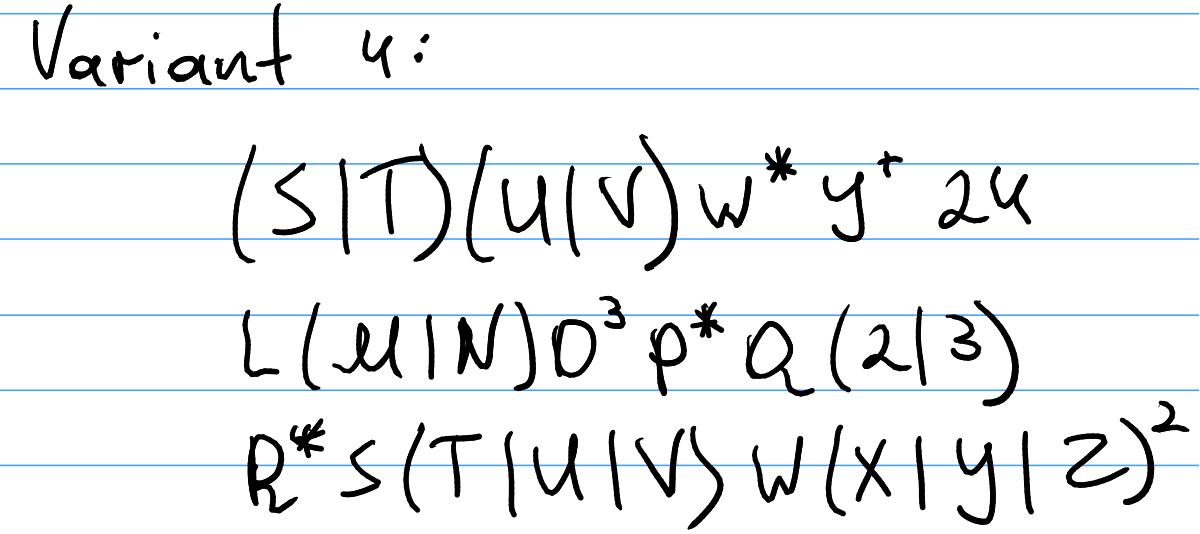
\includegraphics[width=0.78\textwidth]{../variant_4_task.png}
    \end{minipage}

    \vfill
    {\large Chisinau, 2026 \par}
\end{titlepage}

\tableofcontents
\newpage

\section{Abstract}

This laboratory work addresses the problem of dynamically interpreting regular expressions and generating valid strings that conform to them under the constraints of a formal-languages assignment. The goal is not to construct handcrafted output templates for one particular exercise, but rather to engineer a reusable system that can parse multiple regular expressions, convert them into an internal abstract syntax tree, generate valid words, validate those words independently, and explain the generation process step by step.

The implemented solution covers all four assignment variants and all twelve expressions represented by those variants. It includes a normalization layer for handwritten notation, a recursive-descent parser, a bounded generator for languages with potentially infinite repetition, an independent validator based on Python regular expressions, and a visualization subsystem that exports Mermaid-compatible diagrams and generation traces. This transforms the laboratory work from a narrow script into a small, well-structured symbolic language engine.

From an academic perspective, the project demonstrates several important ideas at once: the translation from syntax to structure, the operational interpretation of repetition under bounded conditions, and the role of independent verification in establishing trust in generated results. From an engineering perspective, the system is modular, testable, and explainable. In addition, the report positions the work in dialogue with compiler construction, constraint-based generation, and carefully bounded search in modern sequence systems.

\section{Introduction}

Regular expressions occupy a special place in computer science because they are simultaneously mathematical objects, programming tools, and practical interfaces between human specification and machine behavior. At the formal level, they denote regular languages. At the systems level, they are compiled and executed by engines. At the educational level, they offer a compact and highly expressive medium for understanding symbolic pattern description.

The assignment for this laboratory work asks for more than a superficial use of regular expressions. The requirement is to dynamically interpret the given expressions and generate valid strings accordingly. This is a decisive distinction. A trivial solution would hardcode the output patterns for a specific variant and merely imitate valid samples. Such a solution could print plausible-looking words, but it would fail to solve the general problem. It would neither interpret the symbolic expression nor scale across all variants.

For this reason, the present work adopts a compiler-inspired approach. Each input expression is normalized, parsed, converted into an abstract syntax tree (AST), traversed to generate candidate strings, and validated against an independently emitted regular expression. This architecture makes the implementation universal across variants and provides a principled explanation for each stage of computation.

The work also aims to overachieve relative to the minimum assignment requirements. Beyond dynamic generation, it includes a trace mode that shows how a word was produced, a metric layer that estimates structural complexity, a visualization subsystem for ASTs and traces, and a polished presentation/report package for oral defense. The result is not merely a script that works, but a small formal-language processing pipeline that can be explained, defended, and extended.

\section{Assignment Interpretation and Objectives}

The laboratory brief defines the topic as regular expressions and requires a codebase that can generate valid combinations of symbols according to several complex expressions shown in handwritten form. The core requirement is explicitly dynamic interpretation: the student must give a set of regular expressions as input and obtain valid words as output. The brief additionally states that expressions with unbounded repetition should be limited to at most five expansions, and it offers a bonus point for a function that shows the sequence of processing.

These requirements lead directly to the following engineering objectives:

\begin{enumerate}[label=\arabic*.]
    \item Construct a universal representation for regular expressions that preserves the structure required for generation.
    \item Parse handwritten-style notation reliably, including superscripts and optional whitespace.
    \item Generate valid words without hardcoding expression-specific output templates.
    \item Bound unbounded repetition operators in accordance with the assignment's safety rule.
    \item Validate generated outputs independently so that the generator does not act as its own sole judge.
    \item Expose the generation path through a readable step-by-step trace.
    \item Cover all four variants in one architecture rather than building separate logic per variant.
\end{enumerate}

The resulting system is therefore judged not only by whether it outputs correct words, but also by whether it embodies the correct computational idea. Universality, explainability, and verification are part of the deliverable.

\section{Theoretical Background}

\subsection{Regular Expressions as Descriptions of Regular Languages}

Let $\Sigma$ be a finite alphabet. A regular expression over $\Sigma$ denotes a set of strings, that is, a language $L \subseteq \Sigma^*$. The classical operators used in such descriptions include:

\begin{itemize}
    \item \textbf{concatenation}, where $AB$ denotes strings obtained by taking a string from $A$ followed by a string from $B$;
    \item \textbf{alternation}, where $A|B$ denotes the union of the two languages;
    \item \textbf{Kleene star}, where $A^*$ denotes zero or more repetitions of strings from $A$;
    \item \textbf{plus}, where $A^+$ denotes one or more repetitions of strings from $A$;
    \item \textbf{optionality}, where $A?$ denotes either the empty string or one instance of $A$;
    \item \textbf{exact or bounded powers}, such as $A^n$ or $A\{m,n\}$.
\end{itemize}

While the formal semantics of these operators are well known, the assignment adds an operational rule: if repetition is unbounded, generation must still be finite. This introduces an implementation distinction between the meaning of the language and the strategy used to enumerate representatives from that language.

\subsection{Why an AST is the Right Internal Form}

Parsing expressions directly during generation would be both error-prone and difficult to explain. A more principled architecture separates syntax analysis from execution. The role of the AST is to provide a structural, typed representation of the expression. In this work, every parsed expression is transformed into a tree over four node classes:

\begin{itemize}
    \item \texttt{Literal},
    \item \texttt{Concat},
    \item \texttt{Alternation},
    \item \texttt{Repeat}.
\end{itemize}

This design is important for both correctness and pedagogy. Correctness improves because each operator is handled uniformly once it has been parsed into a typed node. Pedagogy improves because the AST makes it possible to show students and evaluators what structure the machine believes the expression has.

\subsection{Bounded Generation as an Operational Strategy}

The assignment's limit of five for unbounded repetition is best understood as a bounded generation policy, not a redefinition of regex semantics. The language of $A^*$ remains infinite in theory. The engine, however, enumerates a finite subset of it for practical purposes. Formally, if a repeat node has no explicit upper bound, the implementation uses:

\[
\text{upper}(A^*) = \text{max\_repeat}, \qquad \text{upper}(A^+) = \text{max\_repeat}
\]

with the default value \texttt{max\_repeat = 5}. This turns the task into a finite combinatorial problem while preserving the intended acceptance logic.

\section{System Architecture}

The architecture of the system follows a clean, pipeline-oriented design. Each stage has one clear responsibility and communicates through well-defined data structures. This makes the code easier to test, easier to explain during presentation, and easier to extend later.

\begin{figure}[H]
    \centering
    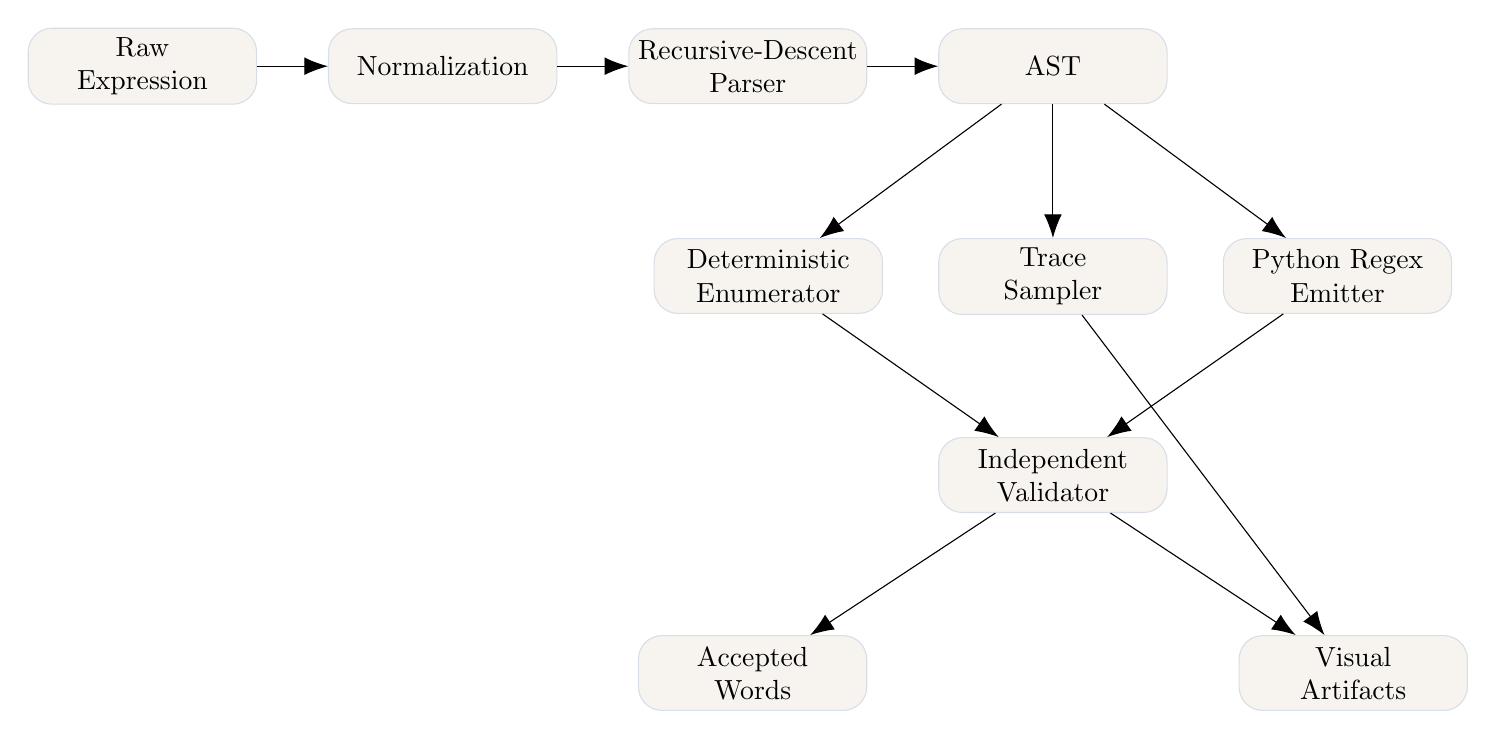
\begin{tikzpicture}[
        node distance=1.55cm and 0.9cm,
        box/.style={draw=labline, rounded corners=3mm, fill=labbg, minimum width=2.9cm, minimum height=0.95cm, align=center},
        >={Latex[length=3mm]}
    ]
        \node[box] (raw) {Raw\\Expression};
        \node[box, right=of raw] (norm) {Normalization};
        \node[box, right=of norm] (parse) {Recursive-Descent\\Parser};
        \node[box, right=of parse] (ast) {AST};
        \node[box, below left=1.7cm and 0.7cm of ast] (enum) {Deterministic\\Enumerator};
        \node[box, below=1.7cm of ast] (trace) {Trace\\Sampler};
        \node[box, below right=1.7cm and 0.7cm of ast] (emit) {Python Regex\\Emitter};
        \node[box, below=of trace] (valid) {Independent\\Validator};
        \node[box, below left=of valid] (words) {Accepted\\Words};
        \node[box, below right=of valid] (diag) {Visual\\Artifacts};

        \draw[->] (raw) -- (norm);
        \draw[->] (norm) -- (parse);
        \draw[->] (parse) -- (ast);
        \draw[->] (ast) -- (enum);
        \draw[->] (ast) -- (trace);
        \draw[->] (ast) -- (emit);
        \draw[->] (enum) -- (valid);
        \draw[->] (emit) -- (valid);
        \draw[->] (trace) -- (diag);
        \draw[->] (valid) -- (words);
        \draw[->] (valid) -- (diag);
    \end{tikzpicture}
    \caption{Processing pipeline of the Lab 4 regular-expression engine.}
\end{figure}

At the module level, the project is organized as follows:

\begin{itemize}
    \item \texttt{src/parser.py}: text normalization and recursive-descent parsing,
    \item \texttt{src/ast\_nodes.py}: typed AST node definitions,
    \item \texttt{src/generator.py}: deterministic and random generation logic,
    \item \texttt{src/visualization.py}: Mermaid-oriented diagram generation and structural metrics,
    \item \texttt{src/variants.py}: universal storage of all assignment variants,
    \item \texttt{main.py}: command-line orchestration.
\end{itemize}

The separation is deliberate. Parsing is not mixed with generation, generation is not mixed with validation, and the assignment data is not mixed with the operational engine.

\section{Parsing and Normalization}

\subsection{Normalization Layer}

The assignment images contain handwritten expressions, which introduces notation that is visually clear to a human but not necessarily explicit enough for a parser. In particular, superscripts such as $^2$ and $^5$ may be represented using Unicode superscript characters, and spaces may appear inconsistently.

The normalization layer solves this by applying three simple but essential transformations:

\begin{enumerate}[label=\arabic*.]
    \item remove whitespace,
    \item convert Unicode superscripts to explicit caret notation,
    \item preserve all other symbolic structure exactly.
\end{enumerate}

This design is intentionally conservative. Normalization does not reinterpret the expression semantically; it only converts surface notation into a stable textual form that the parser can consume deterministically.

\subsection{Recursive-Descent Strategy}

The parser implements a recursive-descent strategy with explicit precedence handling. The precedence hierarchy is:

\[
\text{repetition} \;>\; \text{concatenation} \;>\; \text{alternation}
\]

This is implemented through a stack of parsing functions in which each layer delegates to the next tighter one. The parser begins with alternation, which internally calls concatenation, which in turn calls repetition, which finally calls atomic symbol parsing. This mirrors standard compiler design and keeps each function conceptually small.

\begin{lstlisting}[style=labpython,caption={Representative recursive-descent parsing logic for alternation and concatenation.}]
def _parse_union(self) -> RegexNode:
    options = [self._parse_concat()]
    while self._peek() == "|":
        self._consume("|")
        options.append(self._parse_concat())
    if len(options) == 1:
        return options[0]
    return Alternation(tuple(options))

def _parse_concat(self) -> RegexNode:
    parts = []
    while True:
        token = self._peek()
        if token is None or token in ")|":
            break
        parts.append(self._parse_repetition())
    if not parts:
        return Literal("")
    if len(parts) == 1:
        return parts[0]
    return Concat(tuple(parts))
\end{lstlisting}

The parser also supports:

\begin{itemize}
    \item parenthesized groups,
    \item escaped literals,
    \item exact powers such as \texttt{\^5},
    \item braced quantifiers such as \texttt{\{m,n\}},
    \item epsilon as the empty literal.
\end{itemize}

Invalid syntax is reported through a custom \texttt{RegexSyntaxError}. This is useful not only for debugging, but also for defending the implementation academically: malformed input is rejected explicitly rather than failing silently.

\section{Generation Algorithms}

\subsection{Deterministic Enumeration}

Deterministic generation is the engine's evidence-producing mode. Given an AST, it traverses the structure and enumerates valid words while enforcing two safety conditions:

\begin{itemize}
    \item the number of results is limited by \texttt{max\_results},
    \item unbounded repetition uses the assignment-imposed cap \texttt{max\_repeat = 5}.
\end{itemize}

The implementation is compositional. A literal yields one string. An alternation merges the languages of its options. A concatenation computes pairwise concatenations of partial outputs. A repeat node enumerates allowed counts and expands its child language accordingly.

\begin{lstlisting}[style=labpython,caption={Core idea of deterministic generation for repetition nodes.}]
if isinstance(node, Repeat):
    upper = _upper_repeat_bound(node, max_repeat)
    child_words = generate_language(
        node.node, max_repeat=max_repeat, max_results=max_results
    )
    words = []
    for count in range(node.min_times, upper + 1):
        block = [""]
        for _ in range(count):
            block = _concat_words(block, child_words, max_results)
        words = _merge_unique([*words, *block], max_results)
    return words
\end{lstlisting}

This approach is conceptually straightforward, which makes it appropriate for a teaching-oriented lab. At the same time, the use of uniqueness merging and output limits prevents the algorithm from producing uncontrolled duplication or explosion during normal use.

\subsection{Random Trace Sampling}

The second generation mode creates one valid word together with a trace of how that word was obtained. This mode supports the bonus requirement from the brief: to show the sequence of processing steps.

Each trace step records three fields:

\begin{itemize}
    \item a \textbf{path}, identifying the location in the AST,
    \item an \textbf{action}, such as choosing an alternative or expanding repetition,
    \item a \textbf{detail}, describing the concrete choice made.
\end{itemize}

This design converts the generator from a black box into an explainable symbolic system. For presentation purposes, it also creates a strong narrative bridge between formal grammars and practical tooling.

\section{Independent Validation and Visualization}

\subsection{Validation Through an Independent Backend}

One of the most important design decisions in this laboratory work is the separation between generation and validation. The generator produces candidate strings from the AST. The validator then converts the same AST into a Python-compatible regular expression and checks each candidate using \texttt{re.fullmatch}.

This matters because a generator can accidentally be self-consistent while still being wrong. By validating against an independently emitted formal pattern, the project gains a second source of truth.

\begin{lstlisting}[style=labpython,caption={Validation strategy for generated words.}]
ast = parse_regex(expression)
compiled = re.compile(f"^{to_python_regex(ast)}$")
invalid = [word for word in words if compiled.fullmatch(word) is None]
if invalid:
    raise RuntimeError("Generation mismatch detected.")
\end{lstlisting}

\subsection{Visualization Layer}

The implementation exports Mermaid diagrams for:

\begin{itemize}
    \item AST structure,
    \item high-level processing pipeline,
    \item generation traces.
\end{itemize}

This is especially useful in an oral defense because it allows the invisible symbolic process to be turned into a visible artifact. The report itself uses \LaTeX{} figures for publication quality, while the engine keeps Mermaid output for portability and fast iteration.

\section{Universal Variant Coverage}

The assignment is organized into four variants, each containing three regular expressions. A weak solution would focus only on one of them. The present implementation instead stores all four variants explicitly and interprets all twelve expressions through the same parser and generator.

\subsection{Canonicalized Expressions}

\begin{longtable}{>{\raggedright\arraybackslash}p{1.1cm} >{\raggedright\arraybackslash}p{4.2cm} >{\raggedright\arraybackslash}p{4.8cm} >{\raggedright\arraybackslash}p{4.1cm}}
\caption{Canonicalized machine-readable expressions for all assignment variants.} \\
\toprule
\textbf{Var.} & \textbf{Expression 1} & \textbf{Expression 2} & \textbf{Expression 3} \\
\midrule
\endfirsthead
\toprule
\textbf{Var.} & \textbf{Expression 1} & \textbf{Expression 2} & \textbf{Expression 3} \\
\midrule
\endhead
1 & \texttt{(a|b)(c|d)E+G?} & \texttt{P(Q|R|S)T(UV|W|X)*Z+} & \texttt{1(0|1)*2(3|4)\^5(3)(6)} \\
2 & \texttt{M?N\^2(O|P)\^3Q*R+} & \texttt{(X|Y|Z)\^3(8)+(9|0)} & \texttt{(H|I)(J|K)L*N?} \\
3 & \texttt{O(P|Q|R)+2(3|4)} & \texttt{A*B(C|D|E)F(G|H|I)\^2} & \texttt{J+K(L|M|N)*O?(P|Q)\^3} \\
4 & \texttt{(S|T)(U|V)W*Y+24} & \texttt{L(M|N)O\^3P*Q(2|3)} & \texttt{R*S(T|U|V)W(X|Y|Z)\^2} \\
\bottomrule
\end{longtable}

These expressions are not arbitrary inventions. They are explicit textual interpretations of the handwritten formulas in the assignment. When ambiguities appeared in adjacency or superscript placement, the expressions were grouped explicitly so that parser semantics remained faithful to the shown examples.

\subsection{Variant Task Images}

\begin{figure}[H]
    \centering
    \begin{subfigure}{0.47\textwidth}
        \centering
        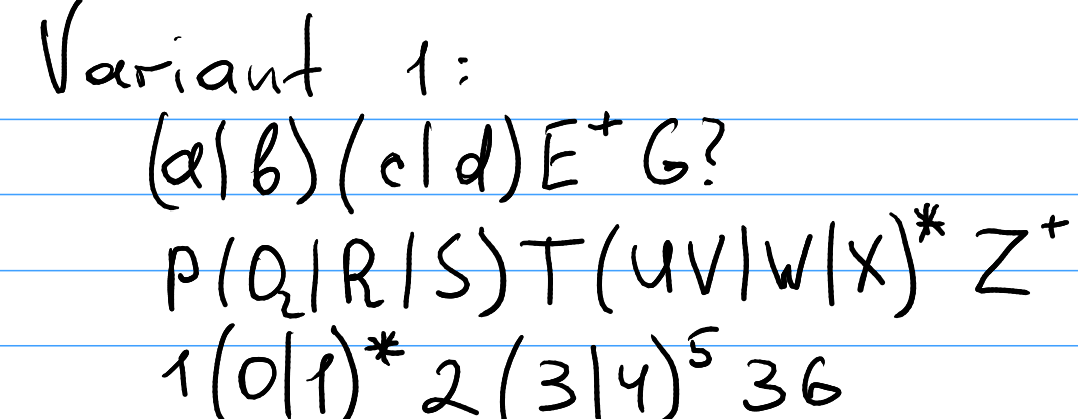
\includegraphics[width=\linewidth]{../variant_1_task.png}
        \caption{Variant 1}
    \end{subfigure}
    \hfill
    \begin{subfigure}{0.47\textwidth}
        \centering
        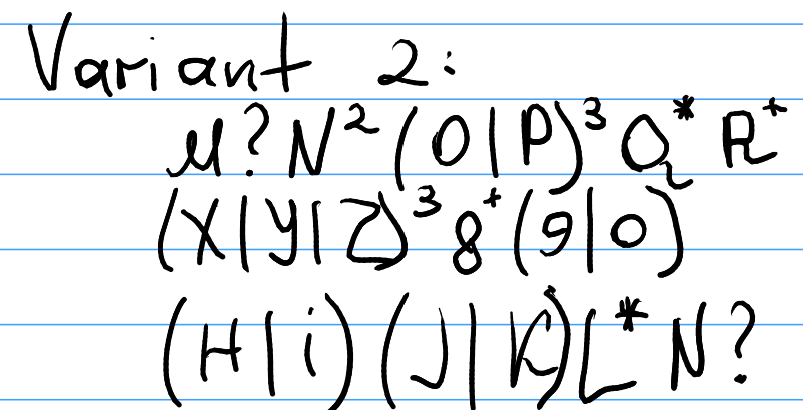
\includegraphics[width=\linewidth]{../variant_2_task.png}
        \caption{Variant 2}
    \end{subfigure}

    \vspace{0.6cm}

    \begin{subfigure}{0.47\textwidth}
        \centering
        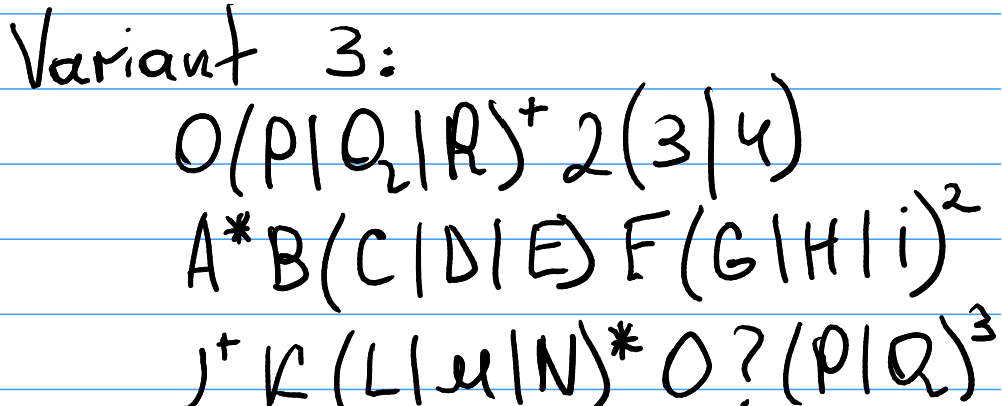
\includegraphics[width=\linewidth]{../variant_3_task.png}
        \caption{Variant 3}
    \end{subfigure}
    \hfill
    \begin{subfigure}{0.47\textwidth}
        \centering
        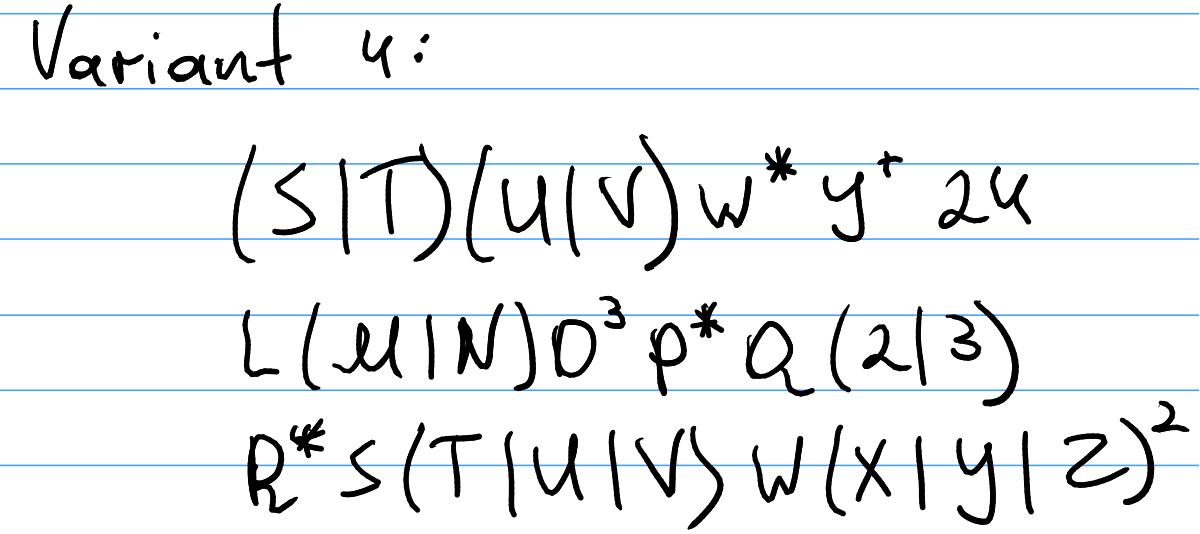
\includegraphics[width=\linewidth]{../variant_4_task.png}
        \caption{Variant 4}
    \end{subfigure}
    \caption{Official assignment variants used as the source specification for the universal generator.}
\end{figure}

\subsection{Variant-by-Variant Discussion}

\textbf{Variant 1} combines front-loaded alternation with both optional and repeated suffix logic. It is a good early test of whether the parser correctly distinguishes between branching and sequential composition. Its third expression additionally verifies exact repetition through the power operator.

\textbf{Variant 2} is notable for its use of exact multiplicities such as $N^2$ and $(O|P)^3$. This makes it comparatively clean from a structural perspective and provides a strong check that exact repetition semantics are implemented correctly.

\textbf{Variant 3} contains the most demanding bounded search space. In particular, the expression \mbox{\texttt{J+K(L|M|N)*O?(P|Q)\^3}} combines mandatory repetition, optionality, alternation, and exact suffix repetition. This expression produces the highest rough path count in the structural analysis.

\textbf{Variant 4} is especially useful in oral presentation because its outputs are visually easy to read. The expression \mbox{\texttt{(S|T)(U|V)W*Y+24}} clearly displays prefix branching, bounded repetition, and a fixed numeric suffix, making it ideal as a pedagogical walkthrough case.

\section{Empirical Analysis Across Variants}

To move beyond anecdotal correctness, the implementation computes structural metrics for every expression. The following table summarizes the main results under the default repeat cap.

\begin{table}[H]
    \centering
    \caption{Structural metrics for all twelve expressions.}
    \begin{tabular}{lrrrrr}
        \toprule
        \textbf{Expr.} & \textbf{Nodes} & \textbf{Depth} & \textbf{Alt.} & \textbf{Repeats} & \textbf{Rough paths} \\
        \midrule
        V1.E1 & 11 & 3 & 2 & 2 & 40 \\
        V1.E2 & 16 & 5 & 2 & 2 & 5460 \\
        V1.E3 & 13 & 4 & 2 & 2 & 2016 \\
        V2.E1 & 13 & 4 & 1 & 5 & 480 \\
        V2.E2 & 11 & 4 & 2 & 2 & 270 \\
        V2.E3 & 11 & 3 & 2 & 2 & 48 \\
        V3.E1 & 11 & 4 & 2 & 1 & 726 \\
        V3.E2 & 14 & 4 & 2 & 2 & 162 \\
        V3.E3 & 15 & 4 & 2 & 4 & 29120 \\
        V4.E1 & 13 & 3 & 2 & 2 & 120 \\
        V4.E2 & 13 & 3 & 2 & 2 & 24 \\
        V4.E3 & 14 & 4 & 2 & 2 & 162 \\
        \bottomrule
    \end{tabular}
\end{table}

The rough path count is not intended as an exact language cardinality. Rather, it is a bounded structural proxy that captures how rapidly the search space can grow when alternation and repetition interact. This proxy highlights the central engineering insight of the project: even in a classroom-sized regex engine, search behavior must be managed explicitly.

\begin{figure}[H]
    \centering
    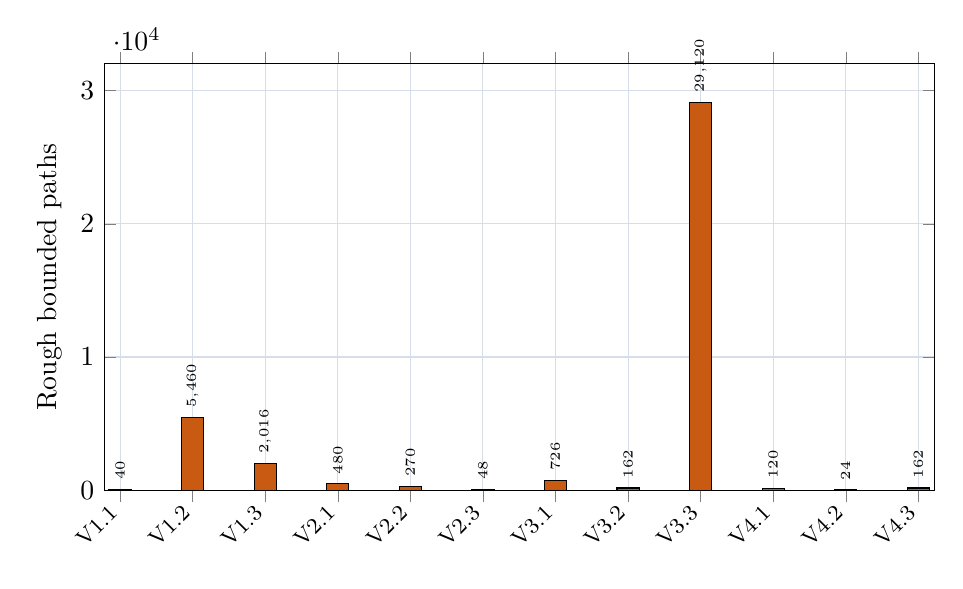
\begin{tikzpicture}
        \begin{axis}[
            width=\textwidth,
            height=7cm,
            ybar,
            bar width=8pt,
            ylabel={Rough bounded paths},
            symbolic x coords={V1.1,V1.2,V1.3,V2.1,V2.2,V2.3,V3.1,V3.2,V3.3,V4.1,V4.2,V4.3},
            xtick=data,
            xticklabel style={rotate=45, anchor=east, font=\footnotesize},
            nodes near coords,
            nodes near coords style={font=\tiny, rotate=90, anchor=west},
            ymin=0,
            enlarge x limits=0.02,
            grid=major,
            grid style={draw=labline},
            major grid style={draw=labline}
        ]
        \addplot[fill=labember] coordinates {
            (V1.1,40) (V1.2,5460) (V1.3,2016)
            (V2.1,480) (V2.2,270) (V2.3,48)
            (V3.1,726) (V3.2,162) (V3.3,29120)
            (V4.1,120) (V4.2,24) (V4.3,162)
        };
        \end{axis}
    \end{tikzpicture}
    \caption{Rough bounded path counts across all expressions. Variant 3, Expression 3 is the dominant outlier.}
\end{figure}

\section{Representative Generated Outputs}

To demonstrate that the generator is not merely syntactically elegant but practically useful, Table \ref{tab:samples} presents representative outputs obtained from the deterministic generator for each variant.

\begin{table}[H]
    \centering
    \caption{Representative generated outputs from the bounded deterministic mode.}
    \label{tab:samples}
    \begin{tabularx}{\textwidth}{lX}
        \toprule
        \textbf{Variant} & \textbf{Representative outputs} \\
        \midrule
        1 & \texttt{acE, acEG, acEE, acEEG, acEEE, acEEEG}; \texttt{PQTZ, PQTZZ, PQTUVZ}; \texttt{123333336, 123333436, 123334336} \\
        2 & \texttt{NNOOOR, NNOOORR, NNOOOQR}; \texttt{XXX89, XXX80, XXX889}; \texttt{HJ, HJN, HJL, HJLLN} \\
        3 & \texttt{OP23, OQ24, OR24}; \texttt{BCFGG, BCFHH, BDFHI}; \texttt{JKPPP, JKPPQ, JKPQQ, JKQPQ} \\
        4 & \texttt{SUY24, SUYY24, SUWY24}; \texttt{LMOOOQ2, LMOOOPQ3, LNOOOPPQ2}; \texttt{STWXX, STWYY, RSTWYZ} \\
        \bottomrule
    \end{tabularx}
\end{table}

These examples support two claims. First, the generator respects the symbolic structure of the expressions, including fixed suffixes and exact powers. Second, the output diversity changes naturally with structural complexity. Expressions with many branches and repeated regions produce visibly richer bounded languages.

\section{Reproducible Evidence Bundle}

To deepen the submission beyond static explanation, the project now includes an evidence-generation pipeline. A single CLI command can regenerate a structured analysis bundle containing:

\begin{itemize}
    \item \texttt{summary.json}: machine-readable metrics, samples, traces, and benchmarks;
    \item \texttt{summary.md}: human-readable analytical summary;
    \item \texttt{terminal\_transcript.txt}: a terminal-style walk-through across all variants.
\end{itemize}

The command used for the run documented in this report was:

\begin{lstlisting}[style=labterminal,caption={Evidence bundle generation command used for this report.}]
python 4_regular_expressions/main.py --variant all --samples 4 --max-results 12 --validate --export-analysis-dir 4_regular_expressions/reports/evidence --benchmark-iterations 5
\end{lstlisting}

This addition strengthens the academic position of the report. Claims about complexity, speed, trace behavior, and validation are no longer only narrative; they are tied to generated artifacts inside the repository itself.

For oral defense and reproducibility, the evidence workflow can be described as a short four-stage protocol:

\begin{enumerate}[label=\arabic*.]
    \item regenerate the analysis bundle from the CLI using the same repeat cap and benchmark settings;
    \item inspect the produced JSON and markdown summaries for structural and timing data;
    \item rerun the automated tests to check behavioral consistency;
    \item rebuild the Slidev deck and PDF report so that the presentation layer matches the measured evidence.
\end{enumerate}

This protocol is intentionally simple. A reviewer does not need private tooling or hidden preprocessing scripts. The repository itself contains the commands and artifacts required to reproduce the main claims.

\section{Benchmark Measurements}

The evidence bundle records lightweight parse, generate, and validate timings for every expression. These measurements are not intended as universal performance claims, since they depend on machine and environment, but they are valuable for relative comparison within this project.

\begin{table}[H]
    \centering
    \caption{Measured benchmark timings in milliseconds from the generated evidence bundle (\texttt{benchmark\_iterations = 5}).}
    \begin{tabular}{lrrr}
        \toprule
        \textbf{Expr.} & \textbf{Parse ms} & \textbf{Generate ms} & \textbf{Validate ms} \\
        \midrule
        V1.E1 & 0.0633 & 0.0526 & 0.0299 \\
        V1.E2 & 0.0537 & 0.0688 & 0.0277 \\
        V1.E3 & 0.0530 & 0.0795 & 0.0291 \\
        V2.E1 & 0.0510 & 0.1464 & 0.0331 \\
        V2.E2 & 0.0922 & 0.0972 & 0.0308 \\
        V2.E3 & 0.0456 & 0.0455 & 0.0342 \\
        V3.E1 & 0.0401 & 0.0450 & 0.0265 \\
        V3.E2 & 0.0583 & 0.0623 & 0.0338 \\
        V3.E3 & 0.0632 & 0.0785 & 0.0337 \\
        V4.E1 & 0.0528 & 0.1528 & 0.0279 \\
        V4.E2 & 0.0724 & 0.0607 & 0.0292 \\
        V4.E3 & 0.0620 & 0.0870 & 0.0323 \\
        \bottomrule
    \end{tabular}
\end{table}

Several observations emerge immediately:

\begin{enumerate}[label=\arabic*.]
    \item Parsing remains uniformly inexpensive across expressions, staying well under $0.1$ ms in the observed run.
    \item Generation cost varies more strongly and reflects structural complexity more clearly than parse cost.
    \item Variant 4, Expression 1 and Variant 2, Expression 1 are among the most expensive generation cases in this measurement set.
    \item Validation is consistently inexpensive relative to generation, which supports the design choice of independent checking after enumeration.
\end{enumerate}

These numbers support an important systems-level conclusion: the main engineering tension in this project is not syntax recognition, but safe traversal of bounded combinatorial structure.

\begin{figure}[H]
    \centering
    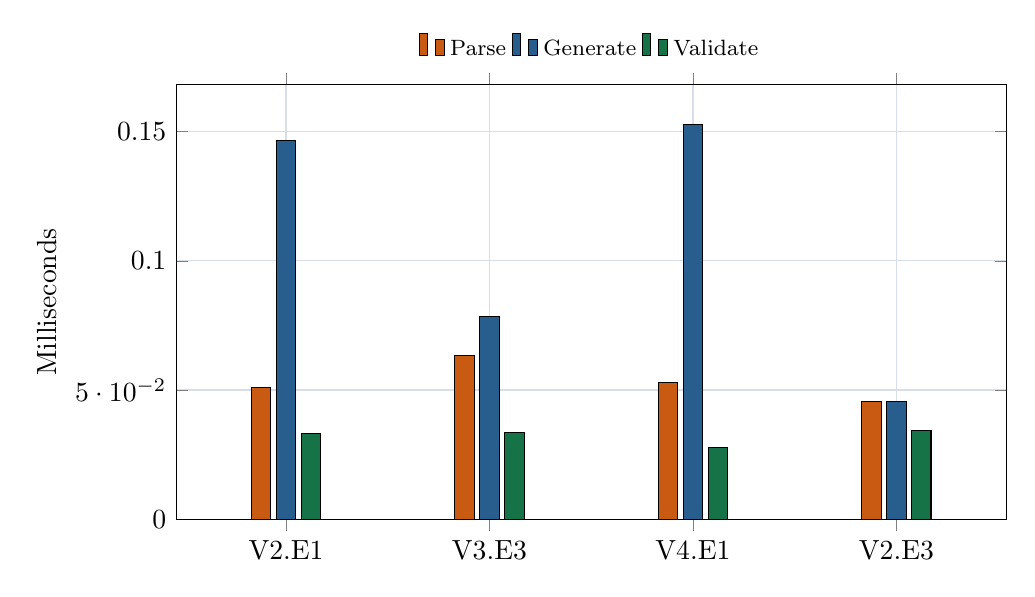
\begin{tikzpicture}
        \begin{axis}[
            width=\textwidth,
            height=7.1cm,
            ybar,
            bar width=7pt,
            ylabel={Milliseconds},
            symbolic x coords={V2.E1,V3.E3,V4.E1,V2.E3},
            xtick=data,
            ymin=0,
            enlarge x limits=0.18,
            grid=major,
            grid style={draw=labline},
            legend style={at={(0.5,1.03)}, anchor=south, legend columns=3, draw=none, fill=none, font=\footnotesize}
        ]
        \addplot[fill=labember] coordinates {(V2.E1,0.0510) (V3.E3,0.0632) (V4.E1,0.0528) (V2.E3,0.0456)};
        \addplot[fill=labblue] coordinates {(V2.E1,0.1464) (V3.E3,0.0785) (V4.E1,0.1528) (V2.E3,0.0455)};
        \addplot[fill=labgreen] coordinates {(V2.E1,0.0331) (V3.E3,0.0337) (V4.E1,0.0279) (V2.E3,0.0342)};
        \legend{Parse, Generate, Validate}
        \end{axis}
    \end{tikzpicture}
    \caption{Representative stage timings. Generation varies far more than parsing or validation.}
\end{figure}

The grouped comparison confirms a qualitative pattern already visible in the table. Parsing remains consistently cheap. Validation also remains cheap. Generation is where structural differences surface operationally. This matters because it explains where engineering effort belongs: not in over-optimizing syntax reading, but in controlling traversal of repeated and branching subtrees.

\section{Complexity, Safety, and Search Behavior}

In the most general case, enumerating strings from a regex-like AST is inherently combinatorial. If a node contains many alternations and repeated substructures, the number of possible outputs grows rapidly. This is not a flaw in the implementation; it is a mathematical property of the language description itself.

Let:

\begin{itemize}
    \item $N$ denote the number of AST nodes,
    \item $B$ denote the effective branching factor introduced by alternation,
    \item $R$ denote the bounded repeat cap used for unbounded operators.
\end{itemize}

Then the number of bounded candidate strings can grow on the order of repeated products and sums involving $B$ and $R$. This is why the system includes:

\begin{enumerate}[label=\arabic*.]
    \item \textbf{repeat capping}, to avoid infinite expansion;
    \item \textbf{max result limiting}, to avoid unbounded output volume;
    \item \textbf{deduplication}, to suppress structural duplication in equivalent generation paths.
\end{enumerate}

The project therefore treats complexity not as an afterthought but as part of the design. This is especially visible in Variant 3, Expression 3, where the structure would be extremely costly to enumerate naïvely.

\section{Correctness Argument}

The project is not a formal proof assistant, but it still benefits from an explicit correctness argument. In a laboratory context, this matters because evaluators need to know not only that outputs look plausible, but also why the pipeline should be trusted.

\subsection{Claim 1: Structure Preservation During Parsing}

After normalization, the parser processes the expression according to a fixed precedence order: repetition, concatenation, then alternation. Each grammar level has a dedicated parsing routine, and each routine constructs only the node types that correspond to that grammatical layer. Because of this design, the produced AST preserves the intended operator nesting of the normalized input.

Informally, the reason this works is classical recursive-descent structure: union parsing delegates to concatenation parsing, concatenation parsing delegates to repetition parsing, and repetition parsing delegates to atom parsing. Since tighter-binding operators are parsed first, the resulting tree respects precedence without requiring ad-hoc repair logic afterward.

\subsection{Claim 2: Soundness of Bounded Generation}

The deterministic generator traverses the AST compositionally. Literals emit fixed symbols, concatenation computes ordered products of child outputs, alternation computes unions of option outputs, and repetition expands a node across an allowed bounded interval. Therefore, every produced candidate is generated by a legal interpretation of the AST under the assignment's repeat cap.

This claim is intentionally phrased as \emph{bounded soundness}. It does not say that the generator enumerates every string in an infinite language. Instead, it says that every emitted string belongs to the intended language once the assignment's finite-generation policy has been applied.

\subsection{Claim 3: Independent Validation of Accepted Outputs}

The generator is not allowed to be its own sole judge. For this reason, the project emits a Python-compatible validation target and checks candidates with full-match semantics. A string is therefore accepted only if it is both generated by the AST traversal and independently recognized by the validation backend.

This dual-check pattern is one of the strongest trust signals in the entire project. Even if a generation bug were introduced, the validator would still serve as an external acceptance filter. Conversely, if the emitted Python regex were malformed, the test suite and example matching checks would detect disagreement between the layers.

\subsection{What This Correctness Story Does and Does Not Guarantee}

The correctness argument supports the following conclusions:

\begin{itemize}
    \item accepted outputs are structurally justified by the AST,
    \item accepted outputs are independently checked against regex semantics,
    \item bounded generation respects the assignment's operational rule for infinite repetition.
\end{itemize}

It does not claim full equivalence with every industrial regex dialect, nor does it claim exhaustive enumeration of infinite languages. Those would be stronger goals than the assignment requires. For the present lab, the relevant result is that the system is sound, explainable, and consistent with the bounded-generation contract.

\section{Verification and Testing}

The repository includes automated tests in both \texttt{tests/test\_lab4\_regex.py} and \texttt{tests/test\_lab4\_analysis.py}. Together they cover the core engine and the evidence-generation layer. The tests cover the following dimensions:

\begin{itemize}
    \item successful parsing of all expressions across all variants,
    \item consistency of official sample strings with interpreted expressions,
    \item agreement between generated outputs and Python regex validation,
    \item correct handling of bounded repetition,
    \item non-empty diagram and metric outputs,
    \item successful generation of step traces,
    \item successful export of the analysis bundle and transcript-oriented summaries.
\end{itemize}

This style of testing is pedagogically significant. It does not merely check one terminal command. Instead, it validates the entire pipeline from syntax analysis through semantic execution to visualization support.

\begin{lstlisting}[style=labpython,caption={Representative test excerpt.}]
def test_star_generation_respects_repeat_limit() -> None:
    node = parse_regex("A*")
    generated = generate_language(node, max_repeat=5, max_results=20)
    assert generated == ["", "A", "AA", "AAA", "AAAA", "AAAAA"]

def test_bonus_trace_returns_steps_and_valid_word() -> None:
    expression = "J+K(L|M|N)*O?(P|Q)^3"
    word, steps = explain_generation(expression, max_repeat=5, seed=7)
    assert word
    assert steps
\end{lstlisting}

The emphasis on independent validation plus testing is one of the strongest aspects of the entire submission. It turns the implementation from a demonstration artifact into a defensible software system.

\subsection{Terminal Transcript Evidence}

The repository now includes a generated transcript in \texttt{reports/evidence/terminal\_transcript.txt}. A representative excerpt is shown below:

\begin{lstlisting}[style=labterminal,caption={Excerpt from the generated evidence transcript.}]
Regular Expressions Lab 4 - analysis transcript
seed=42, max_repeat=5, samples=4, benchmark_iterations=5

VARIANT 3
---------
Expression 3: J+K(L|M|N)*O?(P|Q)^3
Generated: {JKPPP, JKPPQ, JKPQP, JKPQQ}
Task examples: {JJKLOPPP, JKNQQQ}
Metrics: nodes=15, depth=4, alternations=2, repeats=4, rough_paths=29120
Benchmark: parse_ms=0.0632, generate_ms=0.0785, validate_ms=0.0337
Validation target: ^(?:J)+K(?:(?:L|M|N))*(?:O)?(?:(?:P|Q)){3}$
Trace sample: JKNPQP
\end{lstlisting}

This excerpt is useful because it combines the four most important proof dimensions in one place: sample outputs, assignment examples, structural metrics, and performance measurements. It demonstrates that the implementation can produce an integrated analytical view rather than isolated facts.

\section{Threats to Validity and Reproducibility Considerations}

Although the project is carefully engineered, several realism constraints still affect interpretation of the results.

\subsection{Handwritten-to-Canonical Interpretation Risk}

The source assignment variants are handwritten. Before any parser can operate, those formulas must be normalized into explicit machine-readable expressions. This introduces a small interpretation layer in which ambiguous notation must be resolved carefully. The project addresses this risk by documenting the canonicalized forms transparently and by presenting the original task images alongside those forms.

\subsection{Environment-Dependent Benchmark Results}

The benchmark values in this report are reproducible in methodology, but not guaranteed to be identical across machines. Millisecond-level timings depend on processor state, operating system behavior, and Python runtime conditions. For this reason, the benchmarks are used comparatively inside the project, not as universal performance claims.

\subsection{Bounded Enumeration vs Full Language Coverage}

The assignment explicitly authorizes a finite cap for otherwise unbounded repetition. This makes the generator operationally useful, but it also means the generated language is a bounded subset of the full theoretical language when \texttt{*} or \texttt{+} appear. The report therefore distinguishes clearly between regex semantics and the assignment-specific generation policy.

\subsection{Repository-Level Reproducibility}

One of the strongest aspects of the final submission is that its claims remain tied to concrete repository artifacts. The transcript, markdown summary, JSON evidence file, tests, Slidev deck, and PDF report are all generated from the same codebase. This alignment reduces the risk of a mismatch between implementation and presentation.

\section{Discussion and ML/System Analogy}

Although this project is fundamentally a formal-language assignment, it is useful to position it in dialogue with modern systems. The implemented architecture resembles a small symbolic decoding engine:

\begin{itemize}
    \item the AST acts as a symbolic constraint program,
    \item alternation introduces branching possibilities,
    \item bounded repetition acts as a decoding-time regularizer,
    \item independent validation acts as a hard constraint checker.
\end{itemize}

This does \emph{not} mean that the regex generator is equivalent to a neural sequence model. The analogy is more careful than that. It is intended to illuminate a shared systems idea: generation under constraints. In both symbolic and modern ML systems, one often needs to generate outputs while guaranteeing structural correctness.

This analogy is pedagogically useful because it connects formal-language theory with a contemporary engineering intuition. The project remains entirely within the domain of symbolic parsing and generation, but it can still be discussed as a miniature version of constrained decoding logic.

\section{Limitations and Future Work}

No academic report is complete without a realistic account of current limitations. The present implementation intentionally prioritizes correctness, universality, and explainability over feature completeness. Its main limitations are:

\begin{itemize}
    \item it targets the syntax required by the assignment rather than full PCRE-level regex semantics;
    \item it uses bounded generation for infinite operators rather than true language enumeration;
    \item its visualization output is Mermaid-oriented rather than based on a full AST graphics engine;
    \item ambiguity in handwritten notation still requires informed interpretation before canonicalization.
\end{itemize}

These limitations suggest several directions for future work:

\begin{enumerate}[label=\arabic*.]
    \item add support for a richer regex syntax and more robust grouping rules,
    \item compute formal automata from the expressions and compare generation with a separate automaton-based acceptance pipeline,
    \item export diagrams directly to vector formats such as SVG or PDF for publication use,
    \item add performance benchmarking for large bounded enumerations,
    \item integrate an interactive browser dashboard for live classroom exploration.
\end{enumerate}

Such extensions would not change the conceptual core of the project; rather, they would deepen its value as a general educational tool for regular-language processing.

\section{Conclusion}

This laboratory work set out to solve a problem that is easy to underestimate. At a glance, the assignment seems to ask for valid strings that match several regular expressions. In reality, however, it asks for a dynamic interpreter of symbolic specifications. The difference between those two tasks is the difference between imitation and computation.

The final implementation succeeds because it treats the expressions as structured programs. It normalizes handwritten notation, parses it into an AST, generates valid words through bounded traversal, validates those words independently, and exposes the internal reasoning path through traces and diagrams. Most importantly, it does so uniformly across all four variants.

From an academic perspective, the project demonstrates understanding of formal syntax, recursive-descent parsing, bounded search, and regular-language semantics. From a software-engineering perspective, it demonstrates modularity, verification, and explainability. From a presentation perspective, it provides a narrative strong enough to support oral defense and technical discussion.

The strongest claim that can be made about this lab is therefore simple: it is not merely a generator of strings, but a compact, defendable, and reusable regular-expression processing engine.

\appendix

\section{Appendix A - Parser Source Listing}

\lstinputlisting[style=labpython]{../src/parser.py}

\section{Appendix B - Generator Source Listing}

\lstinputlisting[style=labpython]{../src/generator.py}

\section{Appendix C - Visualization Source Listing}

\lstinputlisting[style=labpython]{../src/visualization.py}

\section{Appendix D - Test Suite Listing}

\lstinputlisting[style=labpython]{../tests/test_lab4_regex.py}

\section{Appendix E - Generated Terminal Transcript}

\lstinputlisting[style=labterminal]{evidence/terminal_transcript.txt}

\section{Appendix F - Evidence Summary}

\lstinputlisting[style=labterminal]{evidence/summary.md}

\section{Appendix G - Analysis Module Listing}

\lstinputlisting[style=labpython]{../src/analysis.py}

\section{Appendix H - Analysis Test Listing}

\lstinputlisting[style=labpython]{../tests/test_lab4_analysis.py}

\section{References}

\begin{enumerate}[label={[}\arabic*{]}]
    \item J. E. Hopcroft, R. Motwani, J. D. Ullman, \emph{Introduction to Automata Theory, Languages, and Computation}, Pearson.
    \item M. Sipser, \emph{Introduction to the Theory of Computation}, Cengage Learning.
    \item Python Software Foundation, \emph{re --- Regular expression operations}, \url{https://docs.python.org/3/library/re.html}.
    \item Python Software Foundation, \emph{dataclasses --- Data Classes}, \url{https://docs.python.org/3/library/dataclasses.html}.
    \item Mermaid Documentation, \url{https://mermaid.js.org/}.
    \item Project repository source code and reports contained in the current laboratory workspace.
\end{enumerate}

\end{document}
